\section{Aufbau}
\label{sec:Aufbau}
\begin{figure}
	\centering
	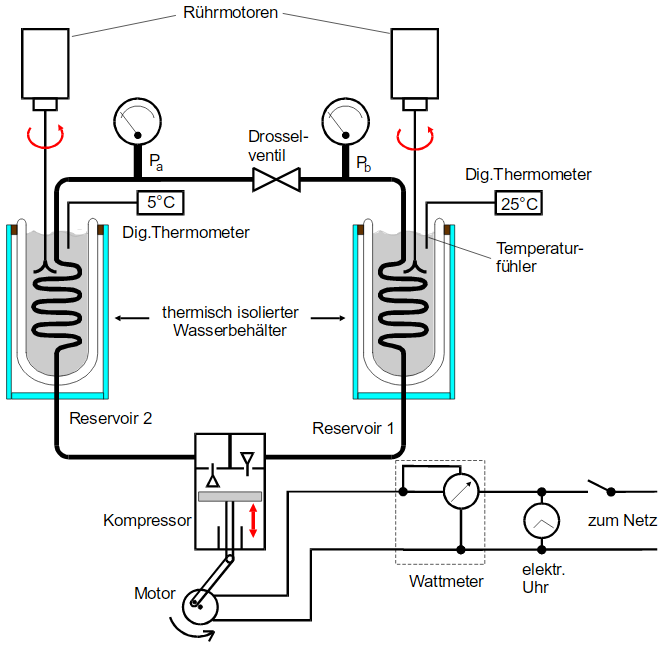
\includegraphics[width=\linewidth-100pt,height=\textheight-100pt,keepaspectratio]{content/Bilder/Aufbau2.png}
	\caption{Expliziter Aufbau der verwendeten Wärmepumpe mit Messapparaturen \cite{V206}.}
	\label{fig:Aufbau2}
\end{figure}
Die in der Messung verwendete Wärmepumpe ist gemäß Abbildung \ref{fig:Aufbau2} aufgebaut. Sie besteht aus zwei thermisch isolierten Wasserbehältern, durch die jeweils ein Kupferrohr, durch welches das Transportgas strömt, spiralförmig verläuft. Im Innerem der Kupferrohrspirale befindet sich jeweils ein Rührer, der von einem Rührmotor angetrieben wird. Zusätzlich befindet jeweils ein Temperatursensor in den Wasserbehältern, sodass $T_1$ im Reservoir 1 und $T_2$ im Reservoir 2 an dem jeweiligen digitalen Thermometer abgelesen werden kann. Auch befindet sich jeweils ein Manometer an jedem der zwei Kupferrohre, um den Druck des Gases $p_\text{b}$ im Reservoir 1 und $p_\text{a}$ im Reservoir 2 messen zu können. Die beiden Kupferrohre sind auf der einen Seite mit einem Drosselventil verbunden und auf der anderen mit einem Kompressor. Die vom Kompressor aufgenommene Leistung wird am Wattmeter angezeigt.